\documentclass[a4paper,12pt, oneside]{article}
\usepackage{geometry} 
\geometry{letterpaper}
\usepackage[parfill]{parskip}
\usepackage{graphicx}
\usepackage{amssymb}
\usepackage{amsmath}
\usepackage[usenames, dvipsnames]{color}
\usepackage{subcaption}
\usepackage [english]{babel}
\usepackage [autostyle, english = american]{csquotes}
\usepackage{float}
\usepackage{verbatim}
\usepackage[normalem]{ulem}
\MakeOuterQuote{"}

\newcommand{\red}[1]{\textcolor{red}{#1}}
\newcommand{\blue}[1]{\textcolor{blue}{#1}}
\newcommand{\green}[1]{\textcolor{green}{#1}}

\usepackage{mathtools}
\newcommand\givenbase[1][]{\:#1\lvert\:}
\let\given\givenbase
\newcommand\sgiven{\givenbase[\delimsize]}
\DeclarePairedDelimiterX\Basics[1](){\let\given\sgiven #1}
\newcommand\Average{E\Basics}

\newcommand*{\myinfinity}{{\propto}}

\title{Thesis Outline -- Very Drafty Draft}
\author{Lizzie Hannah}
\date{\today}

\begin{document}
\maketitle
\section{Abstract}
\section{Introduction}

\blue{Tom comments in blue.}

\green{Things to remove/change are in green.}

\blue{Some terms are repeated very frequently, 
  such as references to Hummel 2003. 
  You should abbreviate it as H3 the first time it's used and
  just use the abbreviation from then on.}
\subsection{History of Flying Discs}
Flying discs have long provided a source of entertainment for dogs and humans alike.  The modern Frisbee -- first produced by Wham-O Inc. toy company in 1957 -- is today a staple in household toy boxes across the United States.  While the precise details of the Frisbee's history continue to be a source of debate, experts generally credit Civil War era baker William Russel Frisbie with designing the baking tin that ultimately became the first Frisbee prototype.  Yale University students purchased Frisbie's pies and played catch by tossing their empty tins around; thus the idea for the Frisbee was borne (1).  

In the late 1940s, Walter Frederick Morrison designed and manufactured the first plastic disc, eventually partnering with Wham-O for mass production and marketing (2). Since then, flying discs have exploded in popularity, providing the basis for sports like Ultimate Frisbee and disc golf. Ultimate Frisbee, a game that combines elements of football and soccer into a fast-paced field sport, is estimated to be played by 7 million people around the globe (4).  Disc golf (as the name suggests) bears many similarities to standard golf: disc golfers compete by throwing discs from "tees" towards targets, aiming to reach the target with as few throws as possible. Though disc sports are relatively young, they are slowly gaining widespread acceptance in the arena of competitive athletics. Indeed, in 2016 the International Olympics Committee granted full recognition to the World Flying Disc Federation, indicating that disc sports may appear in future Olypmic Games (5).

While Wham-O continues to hold a trademark on the term "Frisbee," numerous companies (including Discraft, Innova, EuroDisc, and others) have emerged as competitors in the flying disc market. It is worth mentioning here that, while all flying discs retain the same basic shape, it is possible to observe subtle differences in the trajectories of their flights.  A Frisbee produced by Wham-O, for example, may veer to one direction at the end of a backhand throw, while an Ultrastar produced by Discraft may tail in the opposite direction at the end of a similar throw (3).  As disc sports become increasingly competitive, it will be in the best interest of athletes, coaches, and fans to better understand the aerodynamics of of flying discs.

Despite the recent growth of disc sports, the current body of Frisbee research remains relatively limited. Previous research has developed physics-based models of flying discs, but these models have yet to be refined such that they can predict the flight trajectory of any disc given any set of initial conditions. In particular, the accuracy of the existing models depends heavily on the accuracy of experimental flight data, which is difficult to obtain (2).

\subsection{Motivation for Research}

As mentioned above, understanding the dynamics of Frisbee flight may enable athletes and coaches to improve their performance in sports like Ultimate Frisbee and disc golf.  More generally, however, spinning flying objects display unique and interesting aerodynamic properties, governed by the same principles that guide sophisticated flying vehicles and spacecraft (6). Simply put, a Frisbee is a combination of a wing and a gyroscope. Thus, Bernoulli's Principle (which controls the motion of wings) provides the lift that keeps a Frisbee in the air during flight, and the spin of a Frisbee provides the gyroscopic stability required for a flying disc to maintain its directionality (9). Because of their size and accessibility, Frisbees are convenient objects on which to study patterns of flight in a lab setting. Thus, developing accurate and reliable models of Frisbee throws may prove relevant in designing more complex flying objects. 
 
To date, the most comprehensive model of a thrown disc is described in \textit{Frisbee Flight Simulation and Throw Biomechanics}, published by Sarah Hummel in 2003 (referred to as H3 hereafter). H3 provides a nearly exhaustive review of currently available Frisbee literature and offers a model that builds on the work of (among others) Potts \& Crowther, Yasada, Mitchell, and Stilley \& Carstens (2). 

Ultimately, the goals of this Honors Thesis are twofold. The first goal is to reproduce the model outlined in H3 using a format that is accessible to a relatively wide, general audience, and the second is to test this model against actual flight data obtained from video footage of thrown discs. By reproducing H3's work and refining the model where it fails to match reality, we can add to the existing body of Frisbee literature and help broaden the knowledge of flying disc dynamics for future researchers.

\section{Frisbee Model}

\subsection{Forces}
Understanding the forces and torques that act upon a disc during flight is essential to modeling the trajectory of a Frisbee throw. The following descriptions ignore environmental factors (like wind and rain) that might affect a disc's flightpath, and they further ignore factors such as airflow that could only be accounted for using fluid dynamics. Instead, the forces and torques outlined here appeal to solely classical mechanics in their description of a Frisbee's motion.

Three primary forces influence the translational motion of a flying disc: lift, drag, and gravity (2). Gravity, of course, points vertically downward from the Frisbee's center of mass.  The drag force points in the direction opposite the disc's velocity, working to slow down the Frisbee, and the lift force acts in the direction perpendicular to drag (2). The total force acting on a Frisbee is the sum of all the forces.
\begin{figure}[h]
        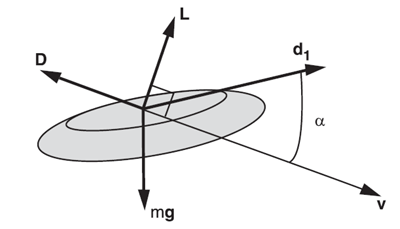
\includegraphics[width=6cm, height=4cm]{frisforces}
	\centering
	\caption{Diagram of forces acting on Frisbee. Note that $\alpha$ denotes angle of attack, the angle between the plane of the disc and the disc's velocity. Figure from Hubbard \& Hummel, 2000}
\end{figure}

To calculate the magnitude of the gravitational force acting on a Frisbee, we simply multiply the mass of a standard Frisbee (0.175 kg) by the constant of gravitational acceleration, here defined as  9.81 $m/s^{2}.$ 
 
The calculation of the lift and drag forces acting on a flying disc, though slightly more complicated than the calculation of the gravitational force, is completed in a similarly standard way. The magnitudes of the lift and drag forces (denoted $F_L$ and $F_D$) are defined by the following equations:

\begin{equation}
  F_D=C_DAv^2\rho/2,
\end{equation}
\begin{equation}
  F_L=C_LAv^2\rho/2
\end{equation}

where \textit{A} is the area of a standard disc (0.057 $m^2$), \textit{v} is the velocity of a thrown disc at time \textit{t}, and $\rho$ is the density of air (taken here to be the average value at sea level of $1.225 kg/m^3$). $C_L$ and $C_D$ represent the coefficients of lift and drag, respectively. Both $C_L$ and $C_D$ are functions of $\alpha$, the angle of attack, defined as the angle between the disc's velocity and the plane of the disc (Figure 1). 

The lift and drag coefficients further depend on a series of parameters that are specific to individual discs (or types of discs); these parameters are constant values that serve to distinguish the trajectory of one Frisbee throw from that of another.  Experiments (\red{include citations here}) show that the drag coefficient has quadratic dependence on $\alpha$, and the lift coefficient has linear dependence on $\alpha$. We will use $\alpha_0$ to denote the value of $\alpha$ at which $F_D$ is at a minimum, here assumed to be $-4^{\circ}$ (2).

\begin{equation}
  C_D=P_{D0}+P_{D\alpha}(\alpha-\alpha_0)^2
\end{equation}
\begin{equation}
  C_L=P_{L0}+P_{L\alpha}\alpha
\end{equation}
\begin{figure}[H]
	\centering
	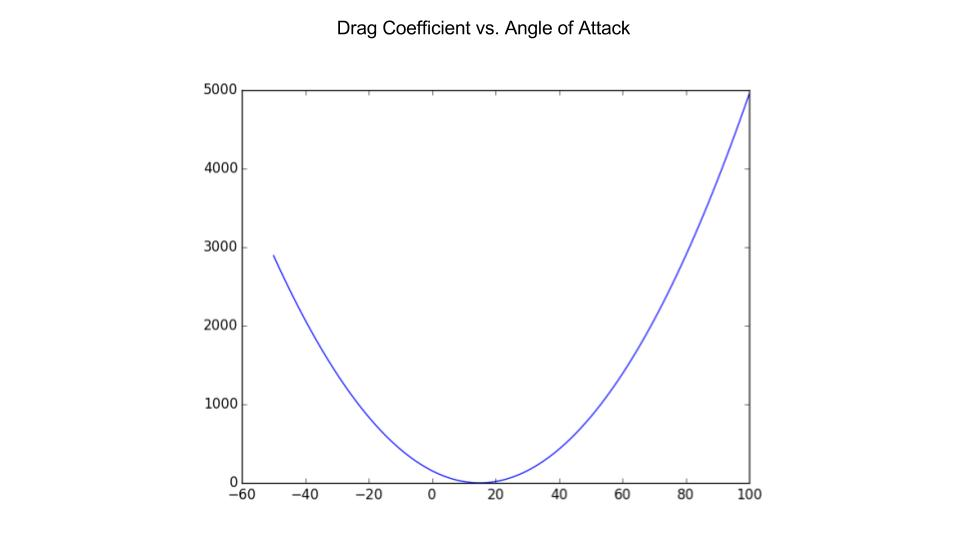
\includegraphics[width=8cm, height=5cm]{DragCoefficientPlot}
	\caption{\color{red}Also include lift vs. angle of attack plot once i figure out how to use the subfigure package. And also make better plots. \color{black}}
\end{figure}
It is these parameters ($P_{D0}, P_{D\alpha}, P_{L0}$, and $P_{L\alpha}$) that form the crux of this Honors Thesis. Previous research has attempted to calculate $P_{D0}, P_{D\alpha}, P_{L0}$, and $P_{L\alpha}$, but to date no consensus on their values exists among the literature (Figure 3). By making small modifications to Hummel's model, the work presented here will offer a parameter estimation method that can be used in future studies.

\begin{figure}[H]
	\centering
	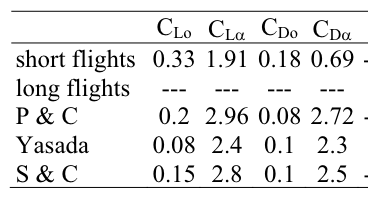
\includegraphics[width=8cm, height=5cm]{ParameterValues}
	\caption{\color{red}Top line is values reported in \blue{H3}. Figure from \blue{H3} \color{black}}
\end{figure}

\subsection{Torques}

In order to produce a representative model of a Frisbee flight in three dimensions, we must refer not only to the forces that act on a flying disc, but also to the torques that cause the disc to rotate about each of its axes. As with the lift and drag forces, the magnitudes of the torques in the \textit{x}, \textit{y}, and \textit{z} directions are calculated using three standard equations that depend on a series of parameters (2 \blue{I think that the original model was NOT proposed by H3. See who see cites as the first to propose it and cite that.}). Here we will use $\tau$ to denote torque.\begin{comment} and we will define $\phi$ to be the angle about the \textit{x}-axis, $\theta$ to be the angle about the \textit{y}-axis, and $\gamma$ to be the angle about the \textit{z}-axis.
\begin{figure}[H]
	\centering
	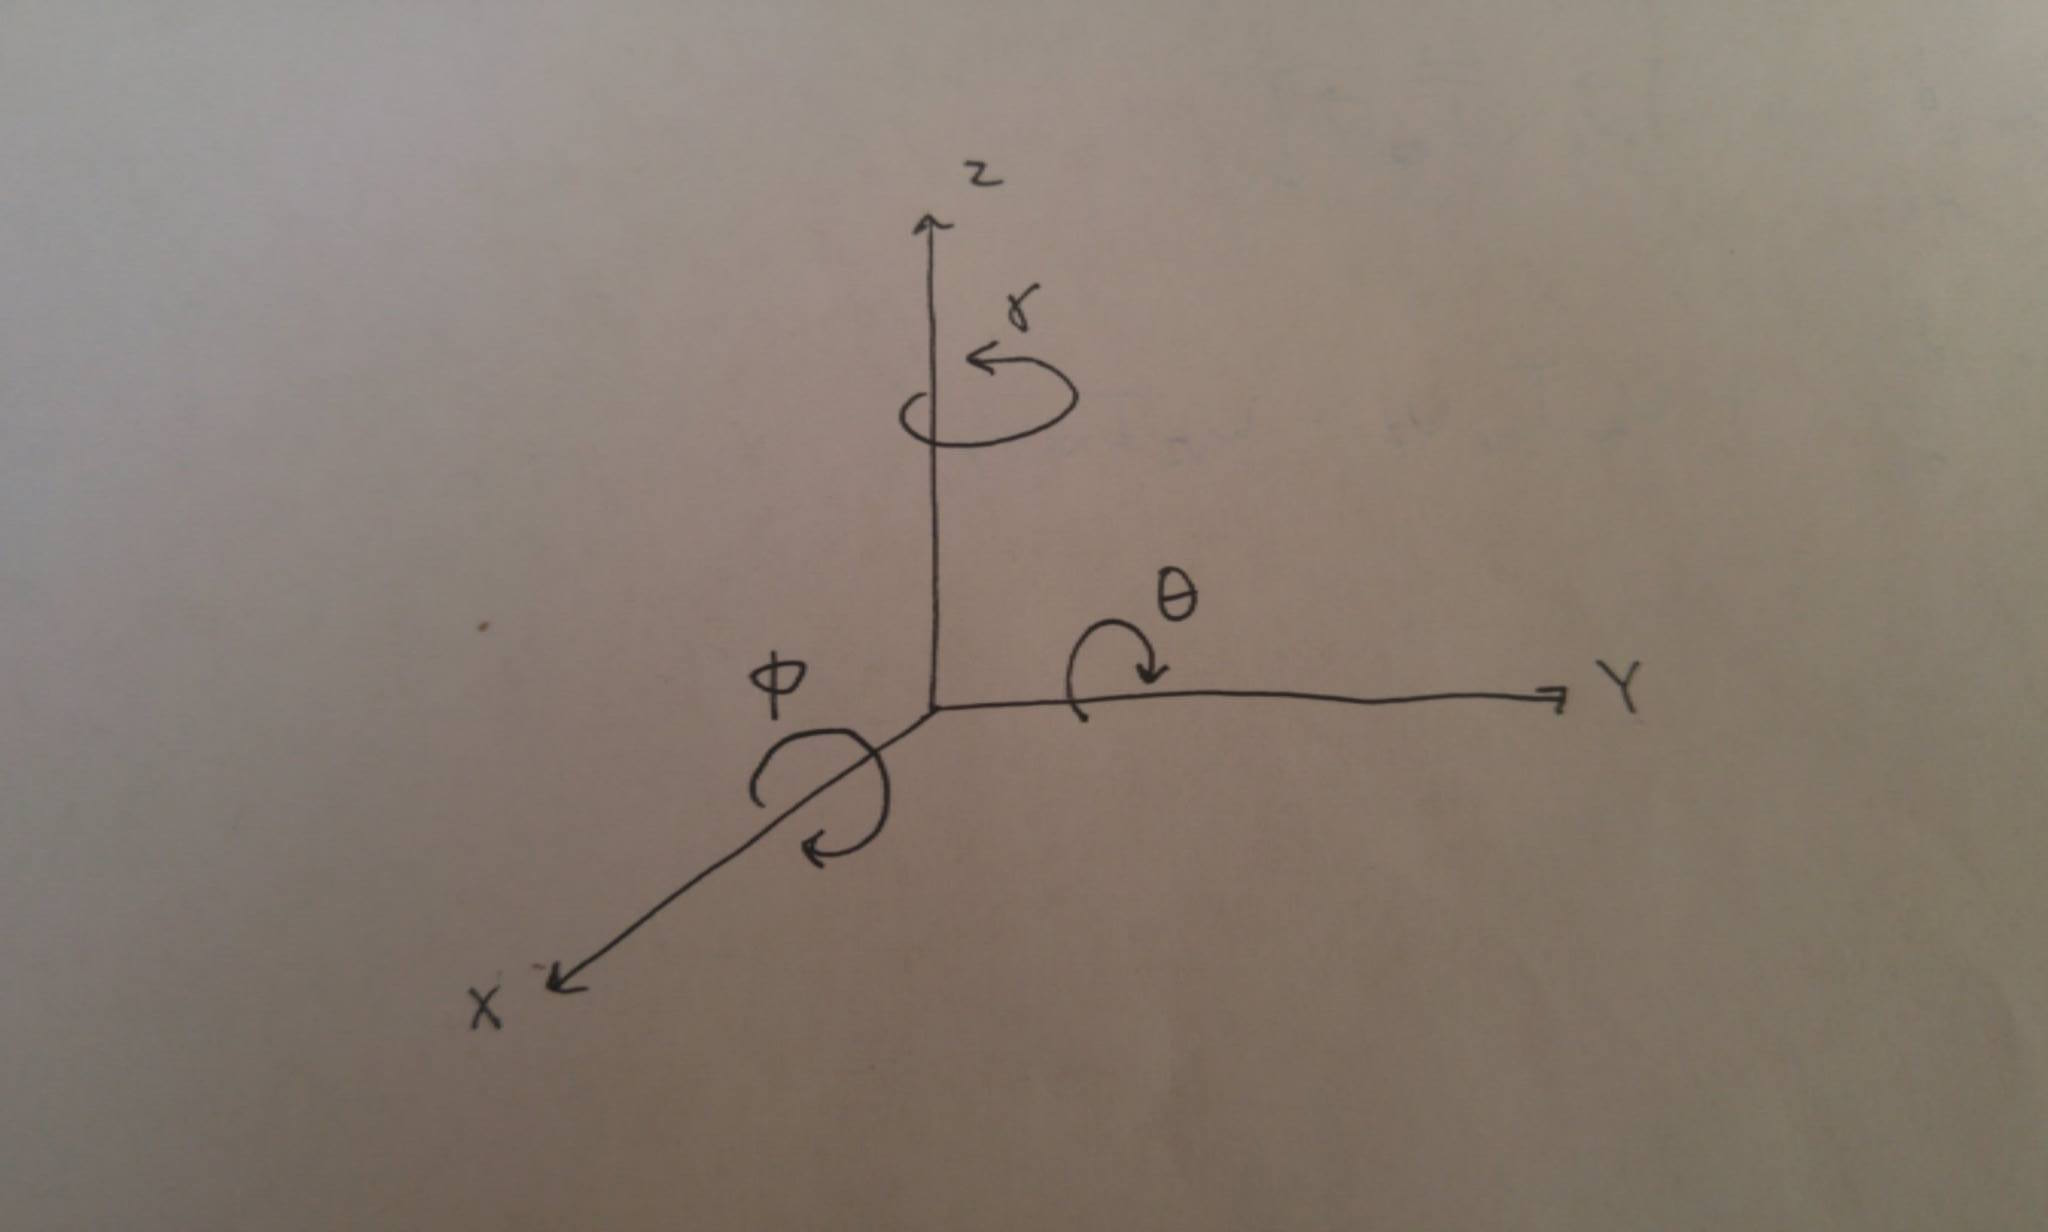
\includegraphics[width=8cm, height=5cm]{AxesDiagram}
	\caption{\red{Fix and make prettier, obvi}}
\end{figure}
\end{comment}

The magnitude of the torque around the \textit{x}-axis depends on two parameters, $P_{\tau_x\omega_x}$ and $P_{\tau_x\omega_z}$, which are multiplied by $\omega_x$ and $\omega_z$, respectively. From here, on $\omega$ denotes angular velocity. According to Hummel, Potts \& Crowther, and others,
\begin{equation}
  \tau_x=(P_{\tau_x\omega_x}\omega_x+P_{\tau_x\omega_z}\omega_z)\frac{1}2Av^2d.
\end{equation}
As before, \textit{A} is the area of a standard disc in m$^2$, \textit{v} is the disc's velocity at time \textit{t}, and \textit{d} is the diameter of a standard disc, here taken to be $\sqrt\frac{1.14}\pi$ m.

Similarly $\tau_y$ and $\tau_z$ are written as,
\begin{equation}
  \tau_y=(P_{\tau_{y0}}+P_{\tau_y\omega_y}\omega_y+P_{\tau_{y\alpha}}\alpha)\frac{1}2Av^2d
\end{equation}
\begin{equation}
  \tau_z=(P_{\tau_z\omega_z}\omega_z)\frac{1}2Av^2d.
\end{equation}

Although this Honors Thesis will attempt to determine the values of the lift and drag parameters, as described above, it will not examine the torque parameters in such thorough detail. For reasons described in the Methods section, it was not possible to obtain accurate experimental data describing the angular positions of a Frisbee during flight. Thus, it was exceedingly difficult to produce meaningful experimental data about torques that could be used for parameter estimation.

\subsection{Newton's Equations of Motion} 

According to classical mechanics, the motion of rigid bodies can be described by two of Newton's equations, which relate an object's translational and rotational trajectory to the sum of the forces and torques acting upon it (7).  The Newton-Euler equations of motion are derived from Newton's two laws of motion for rigid bodies:
\begin{equation}
\vec{F}=\textit{m}\vec{a}
\end{equation}
\begin{equation}
\vec{M}=\dfrac{\vec{dL}}{dt}
\end{equation}
Equation 1 states that the sum of the forces acting upon a rigid body is equal to the product of the body's mass $(\textit{m})$ and its acceleration $(\vec{a})$, where $\vec{a}$ is simply a time derivative of the body's velocity.  

Equation 2 states that a rigid body's angular momentum $(\vec{dL}/dt)$ changes at a rate equal to the sum of the torques $(\vec{M})$ acting upon it. Here we have $\vec{L}$=\textit{I}$\vec{w}$, where \textit{I} is the mass moment of inertia matrix and $\vec{w}$ is the body's angular velocity vector. Due to the axial symmetry of a disc, the inertial matrix for a Frisbee is defined as,  
\begin{equation*}
I=\begin{bmatrix}
I_{xx} & 0 & 0 \\
0 & I_{yy} & 0 \\ 
0 & 0 & I_{zz}
\end{bmatrix},
\end{equation*}
where $I_{xx}$=$I_{yy}$ and $I_{zz}$ is distinct (8).  The nature of $\vec{w}$ depends on a series of rotations that rotate the Frisbee between a standard \textit{xyz} coordinate axis to a new axis, denoted \textit{x'y'z'} (2). These rotations are discussed in the following sections.

\subsection{Euler Rotations} 

Hummel's Frisbee model takes into account several reference frames, which are coordinate systems that describe an object's orientation.  In the following discussion, the term "lab frame" refers to an inertial \textit{x, y, z} reference frame, where the \textit{xy} plane is horizontal and the positive \textit{z} axis points upward.  (Note that H3 defines the +\textit{z} direction to be down, while here we define it to be up.) The term "frisbee frame" refers to a body-fixed coordinate system, \textit{x', y', z'}, in which the \textit{x'y'} plane lies on top of -- or parallel to -- the plane of the Frisbee.

We rotate the coordinates of a disc between the \textit{x,y,z} and \textit{x',y',z',} axes by performing a series of matrix rotations about intermediate sets of axes.  The rotations used here are those described in Hummel (2003), which rotate the Frisbee as follows: 1) about the \textit{x}-axis through angle $\phi$ into an intermediate set of axes denoted $\chi,\eta,\zeta$, 2) about the $\eta$-axis through angle $\theta$ into an intermediate set of axes denoted $\chi',\eta',\zeta'$, and 3) about the $\zeta'$ axis through angle $\gamma$ into \textit{x', y', z'}.

Rotations 1-3 are achieved with three rotation matrices, which can be multiplied together to form a single comprehensive rotation matrix. Rotation 1 can be expressed by the matrix,
\begin{equation*}
C(\phi)=\begin{bmatrix}
1 & 0 & 0 \\
0 & \cos\phi & \sin\phi \\
0 & -\sin\phi & \cos\phi
\end{bmatrix}.
\end{equation*}

Rotation 2 can be expressed by the matrix, 
\begin{equation*}
B(\theta)=\begin{bmatrix}
\cos\theta & 0 & -\sin\theta \\
0 & 1 & 0 \\
\sin\theta & 0 & \cos\theta
\end{bmatrix}.
\end{equation*}

Rotation 3 can be expressed by the matrix, 
\begin{equation*}
D(\gamma)=\begin{bmatrix}
\cos\gamma & \sin\gamma & 0 \\
-\sin\gamma & \cos\gamma & 0 \\
0 & 0 & 1
\end{bmatrix}.
\end{equation*}

In general, we would express the final Euler rotation matrix as a combination of B, C, and D. However, for the purposes of modeling a Frisbee trajectory, we have chosen to rotate the original \textit{x, y, z} axis simply onto the plane of the disc, not onto the spinning disc. This choice was made for the sake of simplifying the model and the numerical calculations it requires (2). Rotating the \textit{x, y, z} axis onto the plane of the disc only requires rotations 1 and 2, which rotate through $\phi$ and $\theta$, respectively.

Therefore, the complete rotation matrix is described as follows:

\begin{equation*}
A(\phi,\theta,\gamma)=A(\phi,\theta)=B(\theta)C(\phi)=\begin{bmatrix}
\cos\theta & \sin\phi\sin\theta & -\sin\theta\cos\phi \\
0 & \cos\phi & \sin\phi \\
\sin\theta & -\sin\phi\cos\theta & \cos\phi\cos\theta
\end{bmatrix}.
\end{equation*}

\subsection{Angular Velocities}
We can denote the angular velocities acting on the Frisbee as $\vec{w}_\phi$, $\vec{w}_\theta$, and $\vec{w}_\gamma$.  According to Goldstein, Poole, \& Safko, these angular velocities point along the "axes that their angles are rotated about."

Consider, for example, $\vec{w}_\phi$.  Before performing any rotations, the vector $(\dot\phi, 0, 0)$ points along the original \textit{x}-axis.  The original \textit{x}-axis is ultimately rotated through angles $\phi$ and $\theta$ via matrices C and B, as described above. In other words, the original \textit{x}-axis undergoes a full transformation by the matrix A$(\phi,\theta)$. Therefore, in order to determine the direction of $\vec{w}_\phi$, we must rotate $(\dot\phi, 0, 0)$ about angles $\phi$ and $\theta$.  This rotation yields:

\begin{equation*}
\vec{w}_\phi=A(\phi,\theta)\left(\begin{array}{ccc}\dot\phi\\0\\0\end{array} \right)=\left(\begin{array}{ccc}\dot\phi\cos\theta\\0\\\dot\phi\sin\theta\end{array} \right).
\end{equation*}

Similarly, in order to find $\vec{w}_\theta$ and $\vec{w}_\gamma$, we can rotate $(0, \dot\theta, 0)$ and $(0, 0, \dot\gamma)$ about the angles through which their original axes are rotated. The vector $(0, \dot\theta, 0)$ originally points along the intermediate $\eta$ axis, which only rotates through the angle $\theta$. As such, we have:
\begin{equation*}
  \vec{w}_\theta=B(\theta)\left(\begin{array}{ccc}
    0\\
    \dot\theta \\
    0
  \end{array} 
  \right)=\left(\begin{array}{ccc}
    0 \\ 
    \dot\theta \\
    0
  \end{array}\right).
\end{equation*}

Since we have only chosen to rotate the original axes of the Frisbee onto the plane of the disc (ignoring spin), the rate at which the angles in the Frisbee frame are changing is equal to the sum $\vec{w}_\phi+\vec{w}_\theta$. Thus,
\begin{equation*}
\vec{w}_F=\left(\begin{array}{ccc}\dot\phi\cos\theta\\\dot\theta\\\dot\phi\sin\theta\end{array} \right)
\end{equation*}

The angular velocity of the Frisbee itself accounts for the final component, $\vec{w}_\gamma$, which already lies along the \textit{z'}-axis after undergoing rotations through $\phi$ and $\theta$. This means that the vector $(0, 0, \dot\gamma)$ does not require any additional rotations, and 
\begin{equation*}
\vec{w}_{Total}=\vec{w}_\gamma+\vec{w}_F=\left(\begin{array}{ccc}\dot\phi\cos\theta\\\dot\theta\\\dot\phi\sin\theta+\gamma\end{array} \right)
\end{equation*}

\subsection{Second Derivative Equations}

Ultimately, grouping Euler's laws of motion together in terms of vectors and matrices yields the Newton-Euler equations of motion (expressed below), which are assumed to govern the flight paths of Frisbees (H3). 
\begin{equation}
\vec{F}=\textit{m}(\dfrac{\vec{dv}}{dt}+\vec{\textit{w}}_F\times\vec{v})
\end{equation}
\begin{equation}
\vec{M}=I\dfrac{\vec{dw}}{dt}+\vec{\textit{w}}_F\times I \vec{w}
\end{equation}

Since we have already written explicit equations for $\textit{w}_F$ and $\textit{w}_{Total}$, we can write the righthand side of Equations 9 and 10 in terms of $\phi$, $\theta$, and $\gamma$. In doing so, we can derive ordinary differential equations (ODEs) that describe both the translational and angular accelerations of a Frisbee throughout its flight. These equations can be numerically integrated in order to determine the position and velocity of a disc at any time during its trajectory. 

First, we calculate $\vec{w}_F\times\vec{v}$: 
\begin{equation*}
\vec{w}_F\times\vec{v}=\left(\begin{array}{ccc} v_z\theta'-v_y(\gamma'+\phi'\sin\theta) \\ v_x(\gamma'+\phi'\sin\theta)-v_z\phi'\cos\theta \\ v_y\phi'\cos\theta-v_x\theta'\end{array}\right).
\end{equation*}

Substituting $\vec{w}_F\times\vec{v}$ into (9), we can solve for acceleration. Thus,

\begin{equation}
\frac{{dv}_x}{dt}=\frac{{F}_x-\theta'v_z+v_y(\phi'\sin\theta)}{m}
\end{equation}

\begin{equation}
\frac{{dv}_y}{dt}=\frac{F_y-v_x\phi'\sin\theta+v_z\phi'\cos\theta}{m}
\end{equation}

\begin{equation}
\frac{{dv}_z}{dt}=\frac{F_z-v_y\phi'\cos\theta+v_x\theta'}{m}
\end{equation}

Next, to solve for angular acceleration, we observe that 
\begin{equation}
  \label{eq:dwdt}
\frac{\vec{dw}}{dt}=\left(\begin{array}{ccc}\ddot\phi\cos\theta-\dot\phi\dot\theta\sin\theta\\ \ddot\theta \\ \ddot\phi\sin\theta + \dot\phi\dot\theta\cos\theta+\ddot\gamma\end{array} \right)
\end{equation}

Substituting (\ref{eq:dwdt}) into (10) and solving for $\ddot\phi$, $\ddot\theta$, and $\ddot\gamma$ yields,
\begin{equation}
\ddot\phi=\frac{M_x-I_{zz}\dot\theta(\dot\phi\sin\theta+\dot\gamma)+2I_{xx}\dot\phi\dot\theta\sin\theta}{I_{xx}\cos\theta}
\end{equation}

\begin{equation}
\ddot\theta=\frac{M_y+I_{zz}\dot\phi\cos\theta(\dot\phi\sin\theta+\dot\gamma)-I_{yy}\dot\phi^2\sin\theta\cos\theta} {I_{yy}}
\end{equation}

\begin{equation}
\ddot\gamma=\frac{M_z-I_{zz}(\dot\phi\dot\theta\cos\theta-\ddot\phi\sin\theta)}{I_{zz}}
\end{equation}

At this point, we see that equations 12-17 are first order ODEs. Indeed, Equations 12, 13, and 14 calculate the translational acceleration of a disc in each direction at time \textit{t}, and Equations 15, 16, and 17 calculate the angular acceleration of a disc at time \textit{t}. Thus, by numerically integrating each of the six equations over a given period of time, we can obtain the velocity of a Frisbee at any point during its flight.

\subsection{Position Coordinates}
\color{BurntOrange}
Once we know the velocity of a flying disc at time \textit{t}, we can perform another series of numerical integrations in order to obtain the position coordinates at time \textit{t}. Letting $\vec{r}=$ denote the \textit{x, y}, and \textit{z} Euclidean positions of a disc during its flight, then 

\begin{equation}
  \label{eq:position_deriv}
  \frac{d\vec{r}}{dt} = \vec{v}.
\end{equation}

Similarly, letting $\phi, \theta$, and $\gamma$ denote the Euler angles of the disc, then
\begin{equation}
\frac{d\phi}{dt}=\dot\phi
\end{equation}
\begin{equation}
\frac{d\theta}{dt}=\dot\theta
\end{equation}
\begin{equation}
\frac{d\gamma}{dt}=\dot\gamma.
\end{equation}
where we obtain $\dot\phi, \dot\theta$, and $\dot\gamma$ via numerical integration of $\ddot\phi, \ddot\theta$, and $\ddot\gamma$. (Likewise, we obtain the components of $\vec{r}$ via numerical integration of $\frac{{dv}_x}{dt}, \frac{{dv}_y}{dt}$, and $\frac{{dv}_z}{dt}$.) It follows, then, that by integrating equations 19-22 over time $t_0$ to $t_f$, we can obtain the Euclidean positions and Euler angles of Frisbee, allowing us to simulate the flight of a flying disc. 

\section{Parameter Estimation}
\subsection{Bayes' Theorem}
In order to estimate the parameters $P_{D0}, P_{D\alpha}, P_{L0}$, and $P_{L\alpha}$, this Honors Thesis will rely on Bayesian statistics. Specifically, we will use Markov Chain Monte Carlo analysis to calculate the probability distribution function of each of the four parameters. 

Bayes' theorem can be expressed as follows:
\begin{equation}
\bold{P}(\theta\given\bold{X})=\frac{\bold{P(\theta})\cdot\bold{P({X}\given\theta})}{\bold{P(\bold{X})}},
\end{equation}
where $\theta$ denotes a set of unknown parameters and $\bold{X}$ denotes a known data set. For our analysis, $\theta$ specifically denotes an array of lift and drag parameters, and $\bold{X}$ denotes a data set obtained from a simulated Frisbee throw, including time, position, and velocity coordinates.

The conditional probability $\bold{P(\theta\given\bold{X})}$ gives the posterior probability distribution of $\bold{\theta}$ given $\bold{X}$. $\bold{P({X}\given\theta})$, in contrast, gives the likelihood of the given data set conditional on certain parameters. $\bold{P(\theta)}$ is known as the prior, which describes any knowledge about $\theta$ that exists in the absence of details regarding $\bold{X}$.

$\bold{P(\bold{X})}$ expresses the likelihood of our known data set $\bold{X}$. In practice we will ignore this term because we cannot determine the likelihood of $\bold{X}$ ahead of time without empirical evidence. Thus, rewriting Bayes' theorem in terms of natural logarithms, we have,
\begin{equation}
\ln\bold{P}(\theta\given\bold{X})=\ln{\bold{P(\theta})+\ln\bold{P({X}\given\theta})}.
\end{equation}

Equation 24 will be used to assess our Frisbee model.
\subsection{Prior Function}
We begin our analysis by defining a prior function ($\bold{P(\theta)}$) that is relevant to our simulated Frisbee throw. In general, this prior function should account for knowledge from past research and physically impossible conditions. However, given the lack of literature surrounding the trajectories of flying discs, such information cannot accurately be incorporated into our analysis.  Thus, because we have relatively little initial knowledge of the values our parameters should take, our model incorporates "flat" priors. 

Based on the results in H3, we suspect the absolute values of $P_{D0}$, $P_{D\alpha}$ and $P_{L0}$, to be less than 1, and we expect the absolute value of $P_{L\alpha}$ to be less than 2. Therefore, we define $\bold{P(\left|\theta\right|>1)}=0$ for $P_{D0}$, $P_{D\alpha}$ and $P_{L0}$, and $\bold{P(\left|\theta\right|>2)}=0$ for $P_{L\alpha}$. When  $\bold{P(\theta)}=0$, $\ln\bold{P(\theta)}=-\infty$. These absolute value restrictions serve as our model's only flat priors.

Our prior function could be made more selective with information about the error measurements obtained by H3, P\&C, and others who have attempted to estimate a Frisbee's lift and drag parameters. For example, given error bars from previous parameter estimations, we could assume the existence of a Gaussian prior. 
\subsection{Likelihood Function}

\color{black}
\section{Works Cited (Tentative)}

1. http://www.wfdf.org/history-stats/history-of-fyling-disc/4-history-of-the-frisbee
2. Hummel thesis \newline
3. Should I cite some sort of observation here? [\blue{Yes, potts and crowther and the others}]\newline
4. http://www.usaultimate.org/about/\newline
5. http://www.wfdf.org/news-media/news/press/2-official-communication/697-international-olympic-committee-grants-full-recognition-to-the-world-flying-disc-federation-wfdf
6. Lorenz 2005 -- Flight and attitude dynamics measurements of an instrumented Frisbee 
\end{document}  
7. Cite a classical mechanics textbook (i.e. NOT wikipedia)
8. Hubbard and Hummel (2000) -- Simulation of Frisbee Flight
9. V.R. Morrison -- The Physics of Frisbees
